

\begin{figure}[h]

\centering






\tikzset{every picture/.style={line width=0.75pt}} %set default line width to 0.75pt        

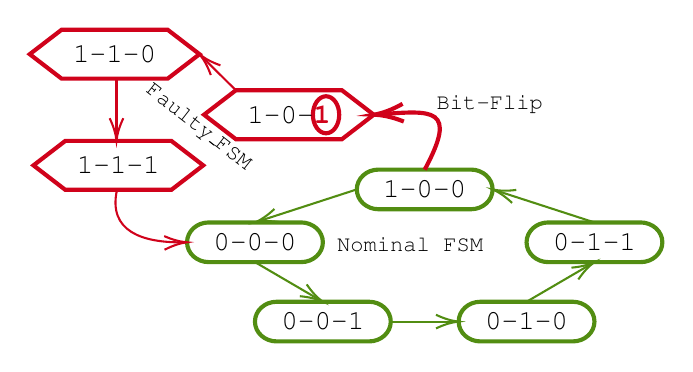
\begin{tikzpicture}[x=0.75pt,y=0.75pt,yscale=-1,xscale=1]
%uncomment if require: \path (0,300); %set diagram left start at 0, and has height of 300

%Flowchart: Terminator [id:dp9084086847868367] 
\draw  [color={rgb, 255:red, 82; green, 141; blue, 18 }  ,draw opacity=1 ][line width=1.5]  (137.18,177.49) -- (181.67,177.49) .. controls (187.46,177.49) and (192.14,181.77) .. (192.14,187.05) .. controls (192.14,192.32) and (187.46,196.6) .. (181.67,196.6) -- (137.18,196.6) .. controls (131.4,196.6) and (126.71,192.32) .. (126.71,187.05) .. controls (126.71,181.77) and (131.4,177.49) .. (137.18,177.49) -- cycle ;
%Flowchart: Terminator [id:dp921126991920133] 
\draw  [color={rgb, 255:red, 82; green, 141; blue, 18 }  ,draw opacity=1 ][line width=1.5]  (235.33,177.49) -- (279.82,177.49) .. controls (285.6,177.49) and (290.29,181.77) .. (290.29,187.05) .. controls (290.29,192.32) and (285.6,196.6) .. (279.82,196.6) -- (235.33,196.6) .. controls (229.54,196.6) and (224.86,192.32) .. (224.86,187.05) .. controls (224.86,181.77) and (229.54,177.49) .. (235.33,177.49) -- cycle ;
%Flowchart: Terminator [id:dp9486811695622979] 
\draw  [color={rgb, 255:red, 82; green, 141; blue, 18 }  ,draw opacity=1 ][line width=1.5]  (268.04,139.28) -- (312.53,139.28) .. controls (318.31,139.28) and (323,143.56) .. (323,148.84) .. controls (323,154.11) and (318.31,158.39) .. (312.53,158.39) -- (268.04,158.39) .. controls (262.26,158.39) and (257.57,154.11) .. (257.57,148.84) .. controls (257.57,143.56) and (262.26,139.28) .. (268.04,139.28) -- cycle ;
%Flowchart: Terminator [id:dp9555553349711161] 
\draw  [color={rgb, 255:red, 82; green, 141; blue, 18 }  ,draw opacity=1 ][line width=1.5]  (186.25,113.81) -- (230.75,113.81) .. controls (236.53,113.81) and (241.21,118.09) .. (241.21,123.36) .. controls (241.21,128.64) and (236.53,132.92) .. (230.75,132.92) -- (186.25,132.92) .. controls (180.47,132.92) and (175.79,128.64) .. (175.79,123.36) .. controls (175.79,118.09) and (180.47,113.81) .. (186.25,113.81) -- cycle ;
%Flowchart: Terminator [id:dp500677861210465] 
\draw  [color={rgb, 255:red, 82; green, 141; blue, 18 }  ,draw opacity=1 ][line width=1.5]  (104.47,139.28) -- (148.96,139.28) .. controls (154.74,139.28) and (159.43,143.56) .. (159.43,148.84) .. controls (159.43,154.11) and (154.74,158.39) .. (148.96,158.39) -- (104.47,158.39) .. controls (98.69,158.39) and (94,154.11) .. (94,148.84) .. controls (94,143.56) and (98.69,139.28) .. (104.47,139.28) -- cycle ;
%Flowchart: Preparation [id:dp3607152634107744] 
\draw  [color={rgb, 255:red, 208; green, 2; blue, 27 }  ,draw opacity=1 ][line width=1.5]  (102.18,87.38) -- (117.51,75.6) -- (168.63,75.6) -- (183.96,87.38) -- (168.63,99.16) -- (117.51,99.16) -- cycle ;
%Straight Lines [id:da8805114399762077] 
\draw [color={rgb, 255:red, 82; green, 141; blue, 18 }  ,draw opacity=1 ][line width=0.75]    (192.14,187.05) -- (222.86,187.05) ;
\draw [shift={(224.86,187.05)}, rotate = 180] [color={rgb, 255:red, 82; green, 141; blue, 18 }  ,draw opacity=1 ][line width=0.75]    (10.93,-3.29) .. controls (6.95,-1.4) and (3.31,-0.3) .. (0,0) .. controls (3.31,0.3) and (6.95,1.4) .. (10.93,3.29)   ;
%Straight Lines [id:da6495626037090436] 
\draw [color={rgb, 255:red, 82; green, 141; blue, 18 }  ,draw opacity=1 ][line width=0.75]    (257.57,177.49) -- (288.56,159.4) ;
\draw [shift={(290.29,158.39)}, rotate = 509.71] [color={rgb, 255:red, 82; green, 141; blue, 18 }  ,draw opacity=1 ][line width=0.75]    (10.93,-3.29) .. controls (6.95,-1.4) and (3.31,-0.3) .. (0,0) .. controls (3.31,0.3) and (6.95,1.4) .. (10.93,3.29)   ;
%Straight Lines [id:da832753655405839] 
\draw [color={rgb, 255:red, 82; green, 141; blue, 18 }  ,draw opacity=1 ][line width=0.75]    (290.29,139.28) -- (243.12,123.98) ;
\draw [shift={(241.21,123.36)}, rotate = 377.98] [color={rgb, 255:red, 82; green, 141; blue, 18 }  ,draw opacity=1 ][line width=0.75]    (10.93,-3.29) .. controls (6.95,-1.4) and (3.31,-0.3) .. (0,0) .. controls (3.31,0.3) and (6.95,1.4) .. (10.93,3.29)   ;
%Straight Lines [id:da7173988733392529] 
\draw [color={rgb, 255:red, 82; green, 141; blue, 18 }  ,draw opacity=1 ]   (175.79,123.36) -- (128.62,138.67) ;
\draw [shift={(126.71,139.28)}, rotate = 342.02] [color={rgb, 255:red, 82; green, 141; blue, 18 }  ,draw opacity=1 ][line width=0.75]    (10.93,-3.29) .. controls (6.95,-1.4) and (3.31,-0.3) .. (0,0) .. controls (3.31,0.3) and (6.95,1.4) .. (10.93,3.29)   ;
%Straight Lines [id:da4444324956160115] 
\draw [color={rgb, 255:red, 82; green, 141; blue, 18 }  ,draw opacity=1 ][line width=0.75]    (126.71,158.39) -- (157.7,176.49) ;
\draw [shift={(159.43,177.49)}, rotate = 210.29] [color={rgb, 255:red, 82; green, 141; blue, 18 }  ,draw opacity=1 ][line width=0.75]    (10.93,-3.29) .. controls (6.95,-1.4) and (3.31,-0.3) .. (0,0) .. controls (3.31,0.3) and (6.95,1.4) .. (10.93,3.29)   ;
%Curve Lines [id:da8286337939248241] 
\draw [color={rgb, 255:red, 208; green, 2; blue, 27 }  ,draw opacity=1 ][line width=1.5]    (208.5,113.81) .. controls (224.68,83.7) and (212.3,85.31) .. (186.79,87.18) ;
\draw [shift={(183.96,87.38)}, rotate = 356.01] [color={rgb, 255:red, 208; green, 2; blue, 27 }  ,draw opacity=1 ][line width=1.5]    (14.21,-4.28) .. controls (9.04,-1.82) and (4.3,-0.39) .. (0,0) .. controls (4.3,0.39) and (9.04,1.82) .. (14.21,4.28)   ;
%Shape: Ellipse [id:dp5162086532146974] 
\draw  [color={rgb, 255:red, 208; green, 2; blue, 27 }  ,draw opacity=1 ][line width=1.5]  (154.63,87.4) .. controls (154.63,82.48) and (157.47,78.48) .. (160.97,78.48) .. controls (164.47,78.48) and (167.31,82.48) .. (167.31,87.4) .. controls (167.31,92.32) and (164.47,96.32) .. (160.97,96.32) .. controls (157.47,96.32) and (154.63,92.32) .. (154.63,87.4) -- cycle ;
%Flowchart: Preparation [id:dp6863452696605052] 
\draw  [color={rgb, 255:red, 208; green, 2; blue, 27 }  ,draw opacity=1 ][line width=1.5]  (18.21,58.22) -- (33.55,46.44) -- (84.67,46.44) -- (100,58.22) -- (84.67,70) -- (33.55,70) -- cycle ;
%Flowchart: Preparation [id:dp4786296734641169] 
\draw  [color={rgb, 255:red, 208; green, 2; blue, 27 }  ,draw opacity=1 ][line width=1.5]  (20,111.78) -- (35.33,100) -- (86.45,100) -- (101.79,111.78) -- (86.45,123.56) -- (35.33,123.56) -- cycle ;
%Straight Lines [id:da32998830369668064] 
\draw [color={rgb, 255:red, 208; green, 2; blue, 27 }  ,draw opacity=1 ]   (60,70) -- (60,98) ;
\draw [shift={(60,100)}, rotate = 270] [color={rgb, 255:red, 208; green, 2; blue, 27 }  ,draw opacity=1 ][line width=0.75]    (10.93,-3.29) .. controls (6.95,-1.4) and (3.31,-0.3) .. (0,0) .. controls (3.31,0.3) and (6.95,1.4) .. (10.93,3.29)   ;
%Straight Lines [id:da0480102553857773] 
\draw [color={rgb, 255:red, 208; green, 2; blue, 27 }  ,draw opacity=1 ]   (117.51,75.6) -- (101.42,59.63) ;
\draw [shift={(100,58.22)}, rotate = 404.78] [color={rgb, 255:red, 208; green, 2; blue, 27 }  ,draw opacity=1 ][line width=0.75]    (10.93,-3.29) .. controls (6.95,-1.4) and (3.31,-0.3) .. (0,0) .. controls (3.31,0.3) and (6.95,1.4) .. (10.93,3.29)   ;
%Curve Lines [id:da1070388681167187] 
\draw [color={rgb, 255:red, 208; green, 2; blue, 27 }  ,draw opacity=1 ]   (60.2,123.8) .. controls (55.93,143.59) and (72.36,149.07) .. (92.15,148.87) ;
\draw [shift={(94,148.84)}, rotate = 538.4300000000001] [color={rgb, 255:red, 208; green, 2; blue, 27 }  ,draw opacity=1 ][line width=0.75]    (10.93,-3.29) .. controls (6.95,-1.4) and (3.31,-0.3) .. (0,0) .. controls (3.31,0.3) and (6.95,1.4) .. (10.93,3.29)   ;

% Text Node
\draw (126.71,148.84) node   [align=left] {{\fontfamily{pcr}\selectfont 0-0-0}};
% Text Node
\draw (159.43,187.05) node   [align=left] {{\fontfamily{pcr}\selectfont 0-0-1}};
% Text Node
\draw (257.57,187.05) node   [align=left] {{\fontfamily{pcr}\selectfont 0-1-0}};
% Text Node
\draw (290.29,148.84) node   [align=left] {{\fontfamily{pcr}\selectfont 0-1-1}};
% Text Node
\draw (208.5,123.36) node   [align=left] {{\fontfamily{pcr}\selectfont 1-0-0}};
% Text Node
\draw (143.07,87.38) node   [align=left] {{\fontfamily{pcr}\selectfont 1-0-\textcolor[rgb]{0.82,0.01,0.11}{\textbf{1}}}};
% Text Node
\draw (212.76,76.15) node [anchor=north west][inner sep=0.75pt]  [font=\footnotesize] [align=left] {{\fontfamily{pcr}\selectfont Bit-Flip}};
% Text Node
\draw (164.76,144.55) node [anchor=north west][inner sep=0.75pt]  [font=\footnotesize] [align=left] {{\fontfamily{pcr}\selectfont Nominal FSM}};
% Text Node
\draw (59.11,58.22) node   [align=left] {{\fontfamily{pcr}\selectfont 1-1-0}};
% Text Node
\draw (60.89,111.78) node   [align=left] {{\fontfamily{pcr}\selectfont 1-1-1}};
% Text Node
\draw (77.68,68.96) node [anchor=north west][inner sep=0.75pt]  [font=\footnotesize,rotate=-38] [align=left] {{\fontfamily{pcr}\selectfont Faulty\_FSM}};



\end{tikzpicture}

\caption{Non Explicit State Exploration Example}
\label{counter}
\end{figure}
